% =========================================================================
%  Smart Threat Detection on Zybo Z7-10 -- Project Presentation Document
%  Paste directly into Overleaf.  Compiles with pdfLaTeX.
% =========================================================================
\documentclass[11pt,a4paper]{article}

% ---------------- Packages -------------------------------------------------
\usepackage[margin=1in]{geometry}
\usepackage{amsmath, amssymb, amsthm}
\usepackage{graphicx}
\usepackage{xcolor}
\usepackage{booktabs}
\usepackage{array}
\usepackage{enumitem}
\usepackage{hyperref}
\usepackage{tikz}
\usepackage{listings}
\usepackage{caption}
\usepackage{fancyhdr}
\usepackage{titlesec}

\usetikzlibrary{arrows.meta, positioning, shapes.geometric, fit, calc,
                decorations.pathreplacing}

% ---------------- Listings setup (VHDL) ------------------------------------
\definecolor{vhdlkw}{RGB}{0,0,170}
\definecolor{vhdltype}{RGB}{30,120,30}
\definecolor{vhdlcom}{RGB}{120,120,120}
\definecolor{vhdlstr}{RGB}{170,30,30}

\lstdefinelanguage{VHDL2008}{
  morekeywords={architecture,entity,is,begin,end,signal,variable,constant,
    port,generic,map,in,out,inout,process,if,then,elsif,else,case,when,
    others,for,loop,to,downto,of,use,library,package,body,return,function,
    procedure,record,type,subtype,array,std_logic,std_logic_vector,unsigned,
    signed,integer,positive,natural,boolean,true,false,null,wait,until,
    rising_edge,falling_edge,attribute,component,configuration,generate,
    range,or,and,not,xor,xnor,nand,nor,with,select,assert,severity,report,
    file,resize,shift_left,shift_right,to_signed,to_unsigned,to_integer,
    work,abs,after,exit,next,open,read_mode,write_mode,append_mode,
    procedure,std,synthesis_off,synthesis_on,inertial,transport},
  sensitive=false,
  morecomment=[l]{--},
  morestring=[b]",
  morestring=[d]'
}

\lstset{
  language=VHDL2008,
  basicstyle=\ttfamily\footnotesize,
  keywordstyle=\color{vhdlkw}\bfseries,
  commentstyle=\color{vhdlcom}\itshape,
  stringstyle=\color{vhdlstr},
  showstringspaces=false,
  numbers=left,
  numberstyle=\tiny\color{gray},
  breaklines=true,
  frame=single,
  rulecolor=\color{black!30},
  tabsize=2,
  captionpos=b,
}

% ---------------- Title page meta ------------------------------------------
\title{
  \vspace{-1cm}
  \textbf{Smart Threat Detection \&\\Situational Awareness System}\\[0.5em]
  \large A pure-VHDL FPGA design on the Digilent Zybo Z7--10
}
\author{Final Project Technical Reference}
\date{}

\pagestyle{fancy}
\fancyhf{}
\fancyhead[L]{Smart Threat Detection -- Zybo Z7--10}
\fancyhead[R]{Technical Reference}
\fancyfoot[C]{\thepage}

\begin{document}
\maketitle
\thispagestyle{empty}

\begin{center}
  \fbox{\parbox{0.92\textwidth}{
    \textbf{One-line summary.}
    A pure programmable-logic VHDL design that fuses ultrasonic distance
    and ambient-light readings, runs them through a six-state threat
    classification FSM, and reports the result on (a) on-board LEDs,
    (b) a Pmod OLED, and (c) an HDMI monitor that draws a polar radar
    sweep with the live target.
  }}
\end{center}

\tableofcontents
\newpage

% ===========================================================================
\section{Project Goal and Constraints}
% ===========================================================================

\subsection{What problem does this solve?}

Detecting an unwanted approach (a person, a vehicle, a moving obstacle)
near a defended asset traditionally relies on a microcontroller polling
several sensors over a network. That introduces latency, OS jitter, and
multi-microsecond worst-case response that is undesirable in
safety-critical applications. The same task is naturally suited to an
FPGA: every sensor sees a dedicated hardware pipeline, every comparator
fires in a single clock cycle, and the response time is bounded by the
physics of the sensor itself.

This project implements such a system on the Digilent
\textbf{Zybo Z7--10} (Xilinx \texttt{xc7z010clg400-1}) using only
programmable logic -- no Zynq Processing System, no AXI, no
microcontroller, no DDR memory, and no Vivado IP cores beyond a small
number of primitive Xilinx cells (\texttt{MMCME2\_BASE},
\texttt{OSERDESE2}, \texttt{OBUFDS}).

\subsection{Hard requirements}

\begin{itemize}[leftmargin=*]
  \item Target part \texttt{xc7z010clg400-1} on a Zybo Z7--10 board.
  \item $\geq 90\%$ of the design expressed as VHDL (no schematic capture, no
        block design except the on-board oscillator pin).
  \item $\geq 2$ Pmod modules driven by the FPGA.
  \item Decision logic implemented as a finite-state machine.
  \item Real-time bound on detection latency: must respond within one
        sensor sampling period.
\end{itemize}

\subsection{Hardware actually used}

\begin{table}[h]
  \centering
  \caption{Pmod modules and on-board peripherals.}
  \begin{tabular}{@{}lll@{}}
    \toprule
    Module & Connector  & Role \\
    \midrule
    Pmod OLED       & JB (12-pin) & SSD1306 status display, 128$\times$32 \\
    Pmod ALS        & JC top row  & ADC081S021 ambient-light sensor (SPI) \\
    Pmod MAXSONAR   & JC bottom row & LV-MaxSonar-EZ1 in PW mode \\
    BTN0 (\texttt{K18}) & on-board & FSM \texttt{start} \\
    BTN3 (\texttt{Y16}) & on-board & FSM \texttt{reset} \\
    LD0--LD3        & on-board & FSM state indicator + alert blink \\
    HDMI TX         & on-board & 640$\times$480@60\,Hz radar visualisation \\
    \bottomrule
  \end{tabular}
\end{table}

% ===========================================================================
\section{High-Level Architecture}
% ===========================================================================

\subsection{System block diagram}

Figure~\ref{fig:block} groups every block in the design by clock domain
and shows the major data paths.

\begin{figure}[h]
\centering
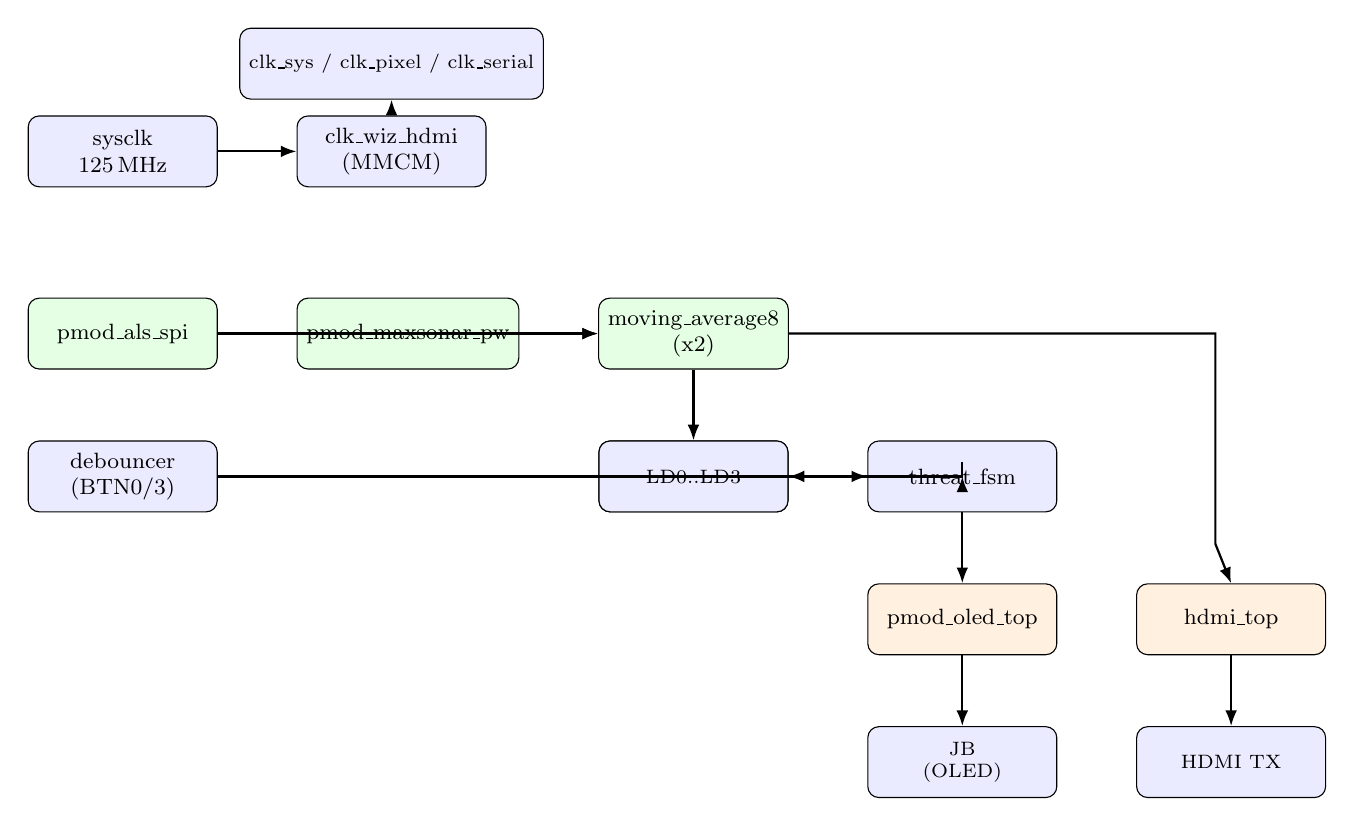
\begin{tikzpicture}[
  node distance=0.9cm and 1.0cm,
  block/.style={draw, rounded corners, fill=blue!8, minimum width=2.4cm,
                minimum height=0.9cm, align=center, font=\footnotesize},
  sblock/.style={block, fill=green!10},
  pblock/.style={block, fill=orange!12},
  arr/.style={-{Latex[length=2mm]}, thick}
]
  % Inputs
  \node[block] (sysclk) {sysclk\\125\,MHz};
  \node[block, right=of sysclk] (mmcm) {clk\_wiz\_hdmi\\(MMCM)};
  \node[block, above=0.2cm of mmcm, font=\scriptsize] (clkout) {clk\_sys / clk\_pixel / clk\_serial};

  % Sensor blocks
  \node[sblock, below=1.4cm of sysclk] (als) {pmod\_als\_spi};
  \node[sblock, right=of als] (sonar) {pmod\_maxsonar\_pw};
  \node[sblock, right=of sonar] (avg) {moving\_average8\\(x2)};

  % Logic blocks
  \node[block, below=of avg] (thr) {threshold\_detect};
  \node[block, right=of thr] (fsm) {threat\_fsm};
  \node[block, below=of als] (btn) {debouncer\\(BTN0/3)};

  % Outputs
  \node[pblock, below=of fsm] (oled) {pmod\_oled\_top};
  \node[pblock, right=of oled] (hdmi) {hdmi\_top};

  \node[block, below=of oled, font=\scriptsize] (jb) {JB\\(OLED)};
  \node[block, below=of hdmi, font=\scriptsize] (hdmiout) {HDMI TX};

  % LED outputs
  \node[block, left=of fsm, font=\scriptsize] (led) {LD0..LD3};

  % wires
  \draw[arr] (sysclk) -- (mmcm);
  \draw[arr] (mmcm) -- (clkout);
  \draw[arr] (als) -- (avg);
  \draw[arr] (sonar) -- (avg);
  \draw[arr] (avg) -- (thr);
  \draw[arr] (thr) -- (fsm);
  \draw[arr] (btn) -| (fsm);
  \draw[arr] (fsm) -- (oled);
  \draw[arr] (avg) -| ($(hdmi.north) + (-0.2,0.5)$) -- (hdmi.north);
  \draw[arr] (fsm) -- (led);
  \draw[arr] (oled) -- (jb);
  \draw[arr] (hdmi) -- (hdmiout);
\end{tikzpicture}
\caption{Block diagram of the top-level design.  Green = sensor pipeline,
blue = control logic, orange = display output.  All sensor blocks live in
the \texttt{clk\_sys} domain; HDMI lives in \texttt{clk\_pixel} (pixels)
and \texttt{clk\_serial} (TMDS bits).}
\label{fig:block}
\end{figure}

\subsection{Data flow in one sentence}

Sensors $\longrightarrow$ filters $\longrightarrow$ thresholds
$\longrightarrow$ FSM $\longrightarrow$ \{LEDs, OLED text, HDMI radar\}.

\subsection{Module inventory}

\begin{table}[h]
  \centering
  \caption{Source files, organised by responsibility.}
  \begin{tabular}{@{}lll@{}}
    \toprule
    Folder            & File                        & Role \\
    \midrule
    \texttt{common/}  & \texttt{synchronizer.vhd}   & 2/3-flop CDC primitive \\
                      & \texttt{debouncer.vhd}      & button stable-window filter \\
                      & \texttt{pulse\_gen.vhd}     & generic strobe generator \\
                      & \texttt{moving\_average8.vhd} & 8-tap box-car filter \\
    \texttt{sensors/} & \texttt{pmod\_als\_spi.vhd} & SPI master, 16-bit frame \\
                      & \texttt{pmod\_maxsonar\_pw.vhd} & PW capture + reciprocal \\
                      & \texttt{threshold\_detect.vhd}  & comparators, generics \\
    \texttt{fsm/}     & \texttt{threat\_fsm.vhd}        & six-state Moore FSM \\
    \texttt{oled/}    & \texttt{oled\_init\_rom.vhd}    & SSD1306 init bytes (pkg) \\
                      & \texttt{font\_5x8\_rom.vhd}     & 5$\times$8 bitmap font (pkg) \\
                      & \texttt{oled\_framebuffer.vhd}  & 512-byte BRAM \\
                      & \texttt{oled\_spi\_master.vhd}  & write-only SPI \\
                      & \texttt{pmod\_oled\_top.vhd}    & power seq + render + refresh \\
    \texttt{hdmi/}    & \texttt{clk\_wiz\_hdmi.vhd}     & MMCM wrapper \\
                      & \texttt{vga\_timing\_640x480.vhd} & H/V counters \\
                      & \texttt{radar\_renderer.vhd}    & per-pixel rasteriser \\
                      & \texttt{tmds\_encoder.vhd}      & DVI 8b/10b \\
                      & \texttt{tmds\_serializer.vhd}   & OSERDESE2 cascade \\
                      & \texttt{hdmi\_top.vhd}          & wires the HDMI pipeline \\
    --                & \texttt{top\_threat\_system.vhd} & top-level integration \\
    \bottomrule
  \end{tabular}
\end{table}

% ===========================================================================
\section{Clocking and Timing Strategy}\label{sec:clk}
% ===========================================================================

\subsection{Why three clock domains}

The design needs three clock frequencies that are not all integer
multiples of each other:

\begin{itemize}
  \item \textbf{System rate.} 125\,MHz is the on-board oscillator and
        is the natural rate for the FSM, sensor SPI, and OLED logic.
        Faster than this is wasted; slower than this loses time
        resolution on the sonar PW capture.
  \item \textbf{Pixel rate.} VGA 640$\times$480@60\,Hz wants
        $800 \times 525 \times 60 = 25.2$\,MHz; the closest
        common-mode clock is exactly 25\,MHz.
  \item \textbf{TMDS serial rate.} DVI/HDMI sends 10 bits per pixel.
        With OSERDESE2 in DDR (2 bits per high-speed clock edge), we
        need a serial clock at $5\times$ the pixel rate, i.e.
        125\,MHz.
\end{itemize}

\subsection{MMCM configuration}

A single \texttt{MMCME2\_BASE} primitive fans the 125\,MHz pin out into
all three clocks.  The maths is:

\begin{align*}
  f_{\text{VCO}} &= f_{\text{in}} \cdot \frac{\text{CLKFBOUT\_MULT\_F}}{\text{DIVCLK\_DIVIDE}}
                  = 125 \cdot \frac{8.0}{1} = 1000~\text{MHz}\\
  f_{\text{pixel}}  &= f_{\text{VCO}} / \text{CLKOUT0\_DIVIDE\_F}  = 1000 / 40   = 25~\text{MHz}\\
  f_{\text{serial}} &= f_{\text{VCO}} / \text{CLKOUT1\_DIVIDE}     = 1000 / 8    = 125~\text{MHz}\\
  f_{\text{sys}}    &= f_{\text{VCO}} / \text{CLKOUT2\_DIVIDE}     = 1000 / 8    = 125~\text{MHz}
\end{align*}

The VCO at 1000\,MHz sits in the centre of the MMCME2 -1
speed-grade range (600--1200\,MHz), giving the cleanest jitter.

\subsection{Reset distribution}

A single asynchronous \emph{cause} (MMCM \texttt{LOCKED} low \emph{or}
power-on counter still counting) feeds into a synchroniser per clock
domain.  This guarantees:

\begin{itemize}
  \item Resets release \emph{after} the MMCM has locked, never before.
  \item Each domain sees its reset edge synchronously to its own clock,
        so flip-flop recovery/removal is met by construction.
  \item No combinational reset reaches an OSERDESE2 (which has timing
        rules on its \texttt{RST} input).
\end{itemize}

\subsection{Cross-domain data}

Only two signals cross from \texttt{clk\_sys} to \texttt{clk\_pixel}: the
filtered sonar distance and the filtered ALS value.  Both are
multi-bit \emph{slowly changing} integers (sonar updates every
$\approx 50$\,ms; ALS every 1\,ms; pixel domain re-samples them only at
60\,Hz vsync).  Two flip-flops with the
\texttt{ASYNC\_REG = "TRUE"} attribute provide adequate
metastability protection -- a Gray-code/handshake structure is
\emph{not} needed because the data is essentially DC-stable between
samples.

\begin{lstlisting}[caption={CDC structure in \texttt{top\_threat\_system.vhd}}]
attribute ASYNC_REG : string;
attribute ASYNC_REG of dist_pix_a : signal is "TRUE";
attribute ASYNC_REG of dist_pix_b : signal is "TRUE";
...
process(clk_pixel)
begin
    if rising_edge(clk_pixel) then
        dist_pix_a <= sonar_filt_out;
        dist_pix_b <= dist_pix_a;
        ...
    end if;
end process;
\end{lstlisting}

The XDC declares the three MMCM outputs as
\texttt{set\_clock\_groups -asynchronous} so Vivado does not try (and
fail) to time the \texttt{sonar\_filt\_out} $\to$ \texttt{dist\_pix\_a}
path.

% ===========================================================================
\section{Sensor Pipeline}
% ===========================================================================

\subsection{Pmod ALS -- ambient light over SPI}

The Pmod ALS hosts a Texas Instruments \texttt{ADC081S021} 8-bit ADC
behind an SPI interface (Mode 0).  A complete read consists of 16 SCLK
cycles:

\begin{itemize}
  \item Cycles 1--3: leading zeros (ADC settling).
  \item Cycles 4--11: 8-bit conversion result, MSB first.
  \item Cycles 12--16: trailing zeros.
\end{itemize}

Our master (\texttt{pmod\_als\_spi.vhd}) drops \texttt{CS\_n}, runs SCLK
at $\approx 1$\,MHz (\texttt{SCLK\_HALF\_CYCLES = 63} at 125\,MHz),
samples MISO on every rising edge into a 16-bit shift register, then
slices out the 8-bit data.  A pulse generator
(\texttt{pulse\_gen}) triggers a new conversion every 1\,ms, giving a
1\,kHz sample rate.

\subsection{Pmod MAXSONAR -- PW capture and integer division}

The MaxBotix LV-MaxSonar-EZ1 outputs a pulse on its PW pin whose
\emph{width} equals the round-trip distance: 147\,$\mu$s per inch.  At
125\,MHz that is

\[
  N_{\text{cyc/inch}} = 147~\mu\text{s} \cdot 125~\text{MHz} = 18\,375
  \text{ cycles per inch.}
\]

So we want the integer division
\[
  \text{inches} = \left\lfloor \frac{N_{\text{cyc}}}{18\,375} \right\rfloor.
\]

A real divider on Zynq-7010 is expensive; a multiply-by-reciprocal
approximation is essentially free.  Pick the largest power of two
that gives an integer multiplier with low error:

\begin{align*}
  R &= \mathrm{round}\!\left(\frac{2^{24}}{18\,375}\right) = 913,\\
  \text{inches} &\approx \left\lfloor \frac{N_{\text{cyc}} \cdot 913}{2^{24}} \right\rfloor
                = (N_{\text{cyc}} \cdot 913) \gg 24.
\end{align*}

\paragraph{Error analysis.}
The exact value of $2^{24}/18\,375$ is $913.04\ldots$, so the relative
error per inch is $0.04 / 913 \approx 4 \times 10^{-5}$.  At the
maximum 254-inch range, the absolute error is below 0.013 inches
(well below the sensor's own 1-inch quantisation).

\paragraph{Watchdog.}
If no rising edge appears within 100\,ms, a watchdog timer emits
\texttt{distance\_in = 0} with \texttt{data\_valid = 1} so downstream
logic does not stall.

\subsection{Filtering: 8-tap moving average}

\texttt{moving\_average8} is a sliding box-car filter that contains no
multipliers.  The running sum is updated incrementally:

\[
  S_{n} = S_{n-1} - x_{n-8} + x_{n}, \qquad
  \bar{x}_{n} = S_{n} \gg 3 \quad (\text{division by 8}).
\]

Eight samples buy roughly 9\,dB of noise reduction on uncorrelated
sensor jitter at the cost of one extra cycle of latency at each new
sample.

% ===========================================================================
\section{Threshold Detection}
% ===========================================================================

\texttt{threshold\_detect.vhd} is a thin combinational block with
registered outputs.  Three thresholds are exposed as VHDL \texttt{generic}
parameters so they can be re-tuned from the top level without recompiling
the leaf module:

\begin{table}[h]
\centering
\begin{tabular}{@{}lll@{}}
\toprule
Generic & Default & Meaning \\ \midrule
\texttt{SONAR\_NEAR\_TH} & 24 & object closer than 24 inches counts as ``near'' \\
\texttt{ALS\_DARK\_TH}   & 32 & ALS reading below 32 counts as ``too dark'' \\
\texttt{ALS\_BRIGHT\_TH} & 220 & ALS above 220 counts as ``too bright'' \\
\bottomrule
\end{tabular}
\end{table}

The block produces five flags consumed by the FSM:

\begin{itemize}
  \item \texttt{sonar\_trig} -- sonar inside the near band.
  \item \texttt{als\_trig}   -- ALS outside its safe band.
  \item \texttt{trig}        -- \texttt{sonar\_trig OR als\_trig}.
  \item \texttt{ok}          -- \texttt{sonar\_trig AND als\_trig} (multi-sensor agreement).
  \item \texttt{conf}        -- \texttt{sonar\_trig AND NOT als\_trig} (single-sensor confirm).
\end{itemize}

% ===========================================================================
\section{The Threat-Detection FSM}
% ===========================================================================

\subsection{Why an FSM, why six states}

An FSM is the natural way to express a multi-step commit policy:
``don't sound the alarm immediately; first hold for a verification
window, then decide whether one sensor is enough or whether we need
both to agree.''  Six states give:

\begin{itemize}
  \item Two \emph{idle} states (\texttt{Idle}, \texttt{Monitor}) so the
        operator can arm the system explicitly.
  \item One \emph{debounce} state (\texttt{Candidate}) that filters out
        transient noise spikes.
  \item One \emph{decision} state (\texttt{Verify}).
  \item Two \emph{commit} states (\texttt{Classify} for severity grading,
        \texttt{Alert} for actually alarming).
\end{itemize}

\subsection{State diagram}

\begin{figure}[h]
\centering
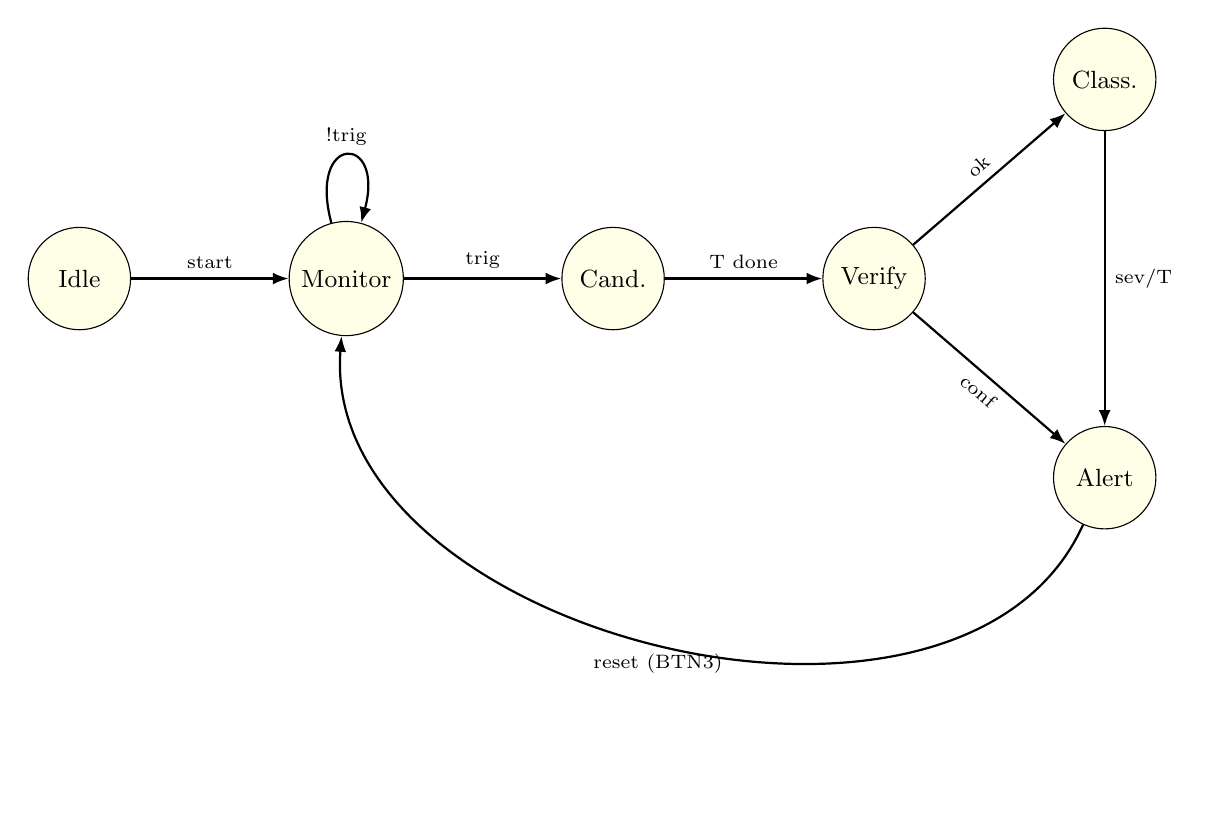
\begin{tikzpicture}[
  node distance=1.6cm and 2.0cm,
  state/.style={draw, circle, fill=yellow!10, minimum size=1.3cm, font=\small},
  arr/.style={-{Latex[length=2mm]}, thick}
]
  \node[state] (idle)  {Idle};
  \node[state, right=of idle] (mon)  {Monitor};
  \node[state, right=of mon]  (cand) {Cand.};
  \node[state, right=of cand] (ver)  {Verify};
  \node[state, above right=of ver] (cls) {Class.};
  \node[state, below right=of ver] (al)  {Alert};

  \draw[arr] (idle) -- node[above, font=\scriptsize] {start} (mon);
  \draw[arr] (mon)  -- node[above, font=\scriptsize] {trig}  (cand);
  \draw[arr] (cand) -- node[above, font=\scriptsize] {T done} (ver);
  \draw[arr] (ver)  -- node[above, sloped, font=\scriptsize] {ok}    (cls);
  \draw[arr] (ver)  -- node[below, sloped, font=\scriptsize] {conf}  (al);
  \draw[arr] (cls)  -- node[right, font=\scriptsize] {sev/T} (al);
  \draw[arr] (al) to[bend left=80] node[below, font=\scriptsize] {reset (BTN3)} (mon);
  \draw[arr] (mon) to[loop above] node[font=\scriptsize] {!trig} ();
\end{tikzpicture}
\caption{FSM transitions.  $T$ is a 100\,ms dwell timer.}
\end{figure}

\subsection{Dwell timer arithmetic}

The dwell timer counts cycles of \texttt{clk\_sys} (125\,MHz).  A
100\,ms hold is therefore
\[
  T_{\text{dwell}} = 100~\text{ms} \cdot 125~\text{MHz}
                   = 12{,}500{,}000~\text{cycles}.
\]
A 24-bit counter is enough; we use 32 bits for code generality.

\subsection{Encoded outputs}

\texttt{state\_code(2:0)} carries a binary encoding so downstream
display modules can mux on it without re-evaluating the case statement:
\(
\text{Idle}{=}000,~\text{Monitor}{=}001,~\text{Candidate}{=}010,~\text{Verify}{=}011,~\text{Alert}{=}100,~\text{Classify}{=}101.
\)

\texttt{severity(1:0)} latches once on the way through \texttt{Verify}
(or \texttt{Classify}): \(00\) for a single-sensor confirm, \(01\) for a
multi-sensor classified threat.  Two bits leave room for future
escalation.

\subsection{LED mapping}

\begin{itemize}
  \item \texttt{LD0}: lit while in \texttt{Idle}.
  \item \texttt{LD1}: lit while in \texttt{Monitor} or \texttt{Candidate}.
  \item \texttt{LD2}: lit while in \texttt{Verify} or \texttt{Classify}.
  \item \texttt{LD3}: blinks at 2\,Hz while in \texttt{Alert}.
\end{itemize}

The 2\,Hz blink is generated by a \texttt{pulse\_gen} (period
$125~\text{MHz}/(125\text{ k} \cdot 250) = 4$\,Hz) toggling a flop, giving
a 2\,Hz square wave.

% ===========================================================================
\section{OLED Display Subsystem}
% ===========================================================================

\subsection{The SSD1306 panel}

The Pmod OLED hosts a Solomon Systech SSD1306 controller driving a
128$\times$32 monochrome OLED panel.  Picking apart the bytes that move
across SPI is straightforward; the \emph{tricky} parts are
(i) the power-up order, (ii) the 100\,ms wait between turning on the
charge pump and turning on the panel high voltage, and (iii) the
horizontal-addressing data layout.

\subsection{Power-up sequencer}

Implemented in \texttt{pmod\_oled\_top.vhd} as a state machine with
four time-gated states followed by two SPI-byte-streaming states:

\begin{enumerate}
  \item \textbf{S\_RESET\_HOLD} -- everything off, RES low, wait 1\,ms.
  \item \textbf{S\_VDD\_ON} -- assert \texttt{VDDC = 0} (logic supply on),
        wait 1\,ms.
  \item \textbf{S\_RES\_LOW} -- pulse RES low for 1\,ms.
  \item \textbf{S\_RES\_HIGH} -- release RES, wait 1\,ms.
  \item \textbf{S\_TX\_INIT\_PRE} -- send 10 init bytes (display off,
        clock-divide, multiplex, offset, start-line, charge-pump enable).
  \item \textbf{S\_VBAT\_ON} -- assert \texttt{VBATC = 0} (panel
        high voltage on), wait \emph{100\,ms}.
  \item \textbf{S\_TX\_INIT\_POST} -- send 16 more init bytes
        (addressing mode, contrast, COM remap, display on \texttt{0xAF}).
\end{enumerate}

The 100\,ms wait between charge pump on and display on is a
hard requirement of the SSD1306 datasheet; skipping it can damage the
OLED panel.

\subsection{Init ROM (\texttt{oled\_init\_rom.vhd})}

A constant array of 32 entries, each \emph{nine bits wide}: bit 8 is the
DC line (\(0 = \text{command}\)), bits 7..0 are the byte payload.
Indices 0..25 are the init sequence; indices 26..31 are the per-frame
prefix (column / page address window) that runs before every refresh.

\subsection{Framebuffer and font}

\texttt{oled\_framebuffer.vhd} is a 512$\times$8 simple dual-port
Block-RAM.  In horizontal addressing mode, byte index $= \text{page}\cdot
128 + \text{col}$; bit 0 of the byte is the topmost pixel of that
8-pixel page.

\texttt{font\_5x8\_rom.vhd} is a function-style ROM returning five
column-major bytes for any printable ASCII character we use
(space, digits, ``:'', ``-'', ``.'', and uppercase letters).  Each
character occupies 6 columns in the framebuffer (5 glyph + 1 spacing),
so each line of 21 characters fits in $6 \cdot 21 = 126$ of the 128
columns -- the trailing two columns stay blank.

\subsection{Render and refresh pipeline}

Every \texttt{REFRESH\_HZ = 30} times per second a refresh tick fires.
The OLED top then walks through:

\begin{enumerate}
  \item \textbf{S\_RUN\_FILL\_TEXT} -- update 15 bytes of the 84-byte
        text buffer with the live state name, distance digits,
        lux digits, and severity digit.
  \item \textbf{S\_RUN\_CLEAR\_FB} -- zero the 512-byte framebuffer
        (so the spacing column between chars is naturally blank).
  \item \textbf{S\_RUN\_RENDER} -- for every (page, char, col-in-glyph)
        tuple, write the glyph byte from the font ROM into the
        framebuffer.
  \item \textbf{S\_RUN\_TX\_PREFIX} -- emit six command bytes
        (column 0..127, page 0..3) so the SSD1306 wraps cleanly.
  \item \textbf{S\_RUN\_TX\_DATA} -- stream all 512 framebuffer bytes
        as data over SPI.
\end{enumerate}

A full refresh costs $\approx 0.85$\,ms at 5\,MHz SPI, $\ll$ the 33\,ms
budget of a 30\,Hz frame, so the OLED is comfortably idle most of the
time.

\subsection{Decimal conversion}

The integer-to-ASCII conversion for the distance and lux numbers is a
combinational helper that uses the synthesizer's built-in
divide-by-constant:

\begin{lstlisting}[caption={Decimal conversion used by the OLED text engine.}]
d := to_integer(distance_in);
if d > 999 then d := 999; end if;
dist_h <= to_unsigned(d / 100, 4);
dist_t <= to_unsigned((d / 10) mod 10, 4);
dist_o <= to_unsigned(d mod 10, 4);
\end{lstlisting}

Vivado folds these constant divisions into a small LUT tree because the
input is bounded.

% ===========================================================================
\section{HDMI Radar Subsystem}
% ===========================================================================

\subsection{Output mode}

We drive the on-board HDMI TX port in \emph{DVI mode} (no audio, no
HDCP, no DDC EDID handshake).  Modern monitors lock cleanly on this if
the source asserts the Hot-Plug-Detect line.  We do that.

The video format is the safest mode in existence:
\(640 \times 480 @ 60~\text{Hz}\), pixel rate exactly 25\,MHz, TMDS
serial rate 125\,MHz.

\subsection{VGA timing block}

\texttt{vga\_timing\_640x480.vhd} is a textbook H/V counter pair.  The
totals come from the VESA 640$\times$480 datasheet:

\[
\begin{array}{l|l|l|l|l|l}
  \text{axis} & \text{active} & \text{front porch} & \text{sync} & \text{back porch} & \text{total} \\
  \hline
  H & 640 & 16 & 96 & 48 & 800 \\
  V & 480 & 10 &  2 & 33 & 525 \\
\end{array}
\]

Both sync pulses are active LOW.  Outputs are \texttt{x}, \texttt{y},
\texttt{de}, \texttt{hsync}, \texttt{vsync}.

\subsection{Per-pixel rasterisation: \texttt{radar\_renderer}}

For every pixel inside the active region we compute, in three pipelined
stages:

\begin{align*}
  \Delta x &= x - c_x, \qquad \Delta y = c_y - y, \qquad (c_x,c_y) = (320,400)\\
  r^2      &= \Delta x^2 + \Delta y^2 \\
  m_{\perp}    &= \Delta x \sin\theta_{\text{sweep}} - \Delta y \cos\theta_{\text{sweep}} \\
  m_{\parallel} &= \Delta x \cos\theta_{\text{sweep}} + \Delta y \sin\theta_{\text{sweep}}
\end{align*}

The pixel colour is then a priority mux over four predicates:

\begin{itemize}
  \item \textbf{Target dot}: a 5$\times$5 box centred on
        $(c_x + r_t \cos\theta_{\text{sweep}},
          c_y - r_t \sin\theta_{\text{sweep}})$ where
        $r_t = 6 \cdot \text{distance\_in}$ pixels per inch.
  \item \textbf{Sweep ray}: $|m_{\perp}| < 2 \cdot 2^{15}$ AND $m_{\parallel} > 0$
        AND $r^2 < R_4^2$.
  \item \textbf{Range ring at radius $R$}: $|r^2 - R^2| \leq R$.
        (This bounds the ring to roughly one-pixel width; deriving from
        the Taylor expansion of $\sqrt{R^2 + \delta} \approx R + \delta/2R$.)
  \item \textbf{Cross-hair}: $x = c_x$ or $y = c_y$.
  \item \textbf{Background}: a dark gray $(8,12,8)$.
\end{itemize}

\subsection{Why a sin/cos LUT and not CORDIC}

We need $\sin\theta$ and $\cos\theta$ at exactly one value per frame
(when the sweep angle advances).  A 64-entry quarter-sine table built
at elaboration time via \texttt{ieee.math\_real} costs nothing in
hardware (Vivado infers it as LUTROM) and provides Q15 precision:
$\sin\theta \in [-32767, 32767]$.

The full circle is reconstructed from quadrant symmetry:

\[
\sin(8\text{-bit }\theta) = \begin{cases}
  +Q[\theta_{[5:0]}]      & \theta_{[7:6]} = 00,\\
  +Q[63 - \theta_{[5:0]}] & \theta_{[7:6]} = 01,\\
  -Q[\theta_{[5:0]}]      & \theta_{[7:6]} = 10,\\
  -Q[63 - \theta_{[5:0]}] & \theta_{[7:6]} = 11.
\end{cases}
\]

$\cos\theta$ is just $\sin(\theta + 64)$ in the same encoding.

\subsection{Sweep advance}

The sweep angle is an 8-bit unsigned counter that increments by 2 on
every \texttt{vsync} edge.  At 60\,Hz that is
$2 \cdot 60 / 256 = 0.47$ revolutions per second, i.e.\ the sweep
crosses a full circle every $\approx 2.13$ seconds.

\subsection{TMDS encoder}

For active video each 8-bit colour component is mapped to a 10-bit TMDS
symbol that satisfies two properties:

\paragraph{Stage 1 -- transition minimisation.}  Reduce 0$\to$1 / 1$\to$0
edges to soften EMI:

\[
  q_{m,0} = D_0,\qquad
  q_{m,i} = q_{m,i-1} \oplus D_i \quad (i=1..7)\quad (\text{XOR mode})
\]

If $D$ has $> 4$ ones, or exactly four ones with $D_0=0$, use XNOR
chaining instead.  $q_{m,8}$ records which mode was used.

\paragraph{Stage 2 -- DC balance.}  Maintain a running disparity
counter so the cumulative number of 1-bits and 0-bits on each TMDS lane
stays balanced (essential for AC-coupled receivers).  The encoder
either passes $q_m$ through or inverts the lower 8 bits and updates the
disparity.

\paragraph{Control symbols.}  During blanking ($de = 0$) the encoder
sends one of four fixed 10-bit patterns derived from
$(c_1, c_0)$ that have very low DC content and a guaranteed run-length
boundary ($\texttt{1101010100}, \ldots$).  Channel 0 (blue) carries
hsync/vsync via $(c_0, c_1)$; channels 1 and 2 fix
$c_0 = c_1 = 0$.

\subsection{Serialiser: OSERDESE2 in 10:1 DDR}

A single OSERDESE2 in DDR mode supports up to an 8:1 ratio.  TMDS needs
10:1, so we cascade a master and a slave:

\begin{itemize}
  \item Master \texttt{OSERDESE2}: \texttt{D1..D8} carry data bits 0..7.
  \item Slave  \texttt{OSERDESE2}: \texttt{D3..D4} carry data bits 8 and 9.
  \item The slave's \texttt{SHIFTOUT1/SHIFTOUT2} feed the master's
        \texttt{SHIFTIN1/SHIFTIN2} via dedicated silicon paths -- no
        timing constraints required.
  \item Master \texttt{OQ} drives an \texttt{OBUFDS} which produces
        the differential pair $(d_p, d_n)$.
\end{itemize}

The clock channel uses the same serialiser fed with the constant
pattern \texttt{1111100000}; that pattern at $f_{\text{serial}}$ is
exactly a square wave at $f_{\text{pixel}}$.

\subsection{Latency budget through the HDMI pipeline}

\begin{table}[h]
\centering
\begin{tabular}{@{}lc@{}}
\toprule
Stage                           & Latency (pixel cycles) \\
\midrule
\texttt{vga\_timing\_640x480}        & 0 (combinational) \\
\texttt{radar\_renderer} stage 1     & 1 \\
\texttt{radar\_renderer} stage 2     & 1 \\
\texttt{radar\_renderer} stage 3     & 1 \\
\texttt{tmds\_encoder}                & 1 \\
\texttt{tmds\_serializer}             & 2--3 (OSERDES internal) \\
\bottomrule
\end{tabular}
\end{table}

The hsync/vsync signals are pipelined alongside the colour data so
they hit the encoder in lock-step with the pixels they describe.

% ===========================================================================
\section{Top-Level Integration}
% ===========================================================================

The \texttt{top\_threat\_system.vhd} file is intentionally thin -- it
contains no logic of its own beyond reset/clock distribution and a few
LED muxes.  Everything else is delegated to the leaf modules.

\begin{lstlisting}[caption={Top-level fan-out (abbreviated).}]
clk_wiz_i : entity work.clk_wiz_hdmi
    port map (clk_in => sysclk, ...,
              clk_sys => clk_sys, clk_pixel => clk_pixel,
              clk_serial => clk_serial, locked => mmcm_locked);
...
sonar_inst : entity work.pmod_maxsonar_pw    -- on clk_sys
    port map (...);
fsm_inst   : entity work.threat_fsm          -- on clk_sys
    port map (...);
oled_inst  : entity work.pmod_oled_top       -- on clk_sys
    port map (...);
hdmi_inst  : entity work.hdmi_top            -- on clk_pixel + clk_serial
    port map (..., distance_in => dist_pix_b, als_value => als_pix_b, ...);
\end{lstlisting}

% ===========================================================================
\section{Constraints (XDC)}
% ===========================================================================

\subsection{Pin map}

Every pin in \texttt{xdc/zybo\_z7\_10.xdc} is taken from the official
Digilent Zybo Z7--10 master XDC.  Highlights:

\begin{table}[h]
\centering
\begin{tabular}{@{}lll@{}}
\toprule
Signal              & Pin   & I/O Std       \\
\midrule
\texttt{sysclk}     & K17   & LVCMOS33      \\
\texttt{btn\_start} & K18   & LVCMOS33      \\
\texttt{btn\_reset} & Y16   & LVCMOS33      \\
\texttt{led[0..3]}  & M14, M15, G14, D18 & LVCMOS33 \\
JB OLED pins        & V8/W8/V7/Y7/Y6/V6/W6 & LVCMOS33 \\
JC ALS pins         & V15/T11/T10 & LVCMOS33 \\
JC sonar pin        & T12   & LVCMOS33      \\
HDMI TX clock pair  & H16/H17 & TMDS\_33   \\
HDMI TX data pairs  & D19/D20, C20/B20, B19/A20 & TMDS\_33 \\
\bottomrule
\end{tabular}
\end{table}

\subsection{Asynchronous clock groups}

\begin{lstlisting}[language=tcl, caption={CDC handling in the XDC.}]
set_clock_groups -asynchronous \
    -group [get_clocks -include_generated_clocks sys_clk_pin] \
    -group [get_clocks -of_objects [get_pins ... mmcm_i/CLKOUT0]] \
    -group [get_clocks -of_objects [get_pins ... mmcm_i/CLKOUT1]] \
    -group [get_clocks -of_objects [get_pins ... mmcm_i/CLKOUT2]]
\end{lstlisting}

This tells Vivado that paths between any two of these clocks are not
to be constrained -- exactly correct given that we cross with
\texttt{ASYNC\_REG} synchronisers.

% ===========================================================================
\section{Build and Verification Flow}
% ===========================================================================

\subsection{Vivado non-project flow}

\texttt{scripts/build.tcl} drives Vivado in batch mode without a
\texttt{.xpr} project file:

\begin{lstlisting}[language=tcl, caption={Skeleton of \texttt{build.tcl}.}]
read_vhdl -vhdl2008 src/rtl/oled/oled_init_rom.vhd
read_vhdl -vhdl2008 ...    ;# (every RTL source, ordered for packages)
read_xdc xdc/zybo_z7_10.xdc

synth_design -top top_threat_system -part xc7z010clg400-1
opt_design
place_design
phys_opt_design
route_design
write_bitstream -force build/threat_system.bit
\end{lstlisting}

The reproducibility benefit is huge: every build is a single command and
its checkpoints, utilisation report, and timing summary land in
\texttt{build/}.

\subsection{Testbench coverage}

\begin{table}[h]
\centering
\begin{tabular}{@{}ll@{}}
\toprule
Testbench & Asserts \\
\midrule
\texttt{tb\_synchronizer}     & latency $\equiv$ STAGES; reset reloads RST\_VAL \\
\texttt{tb\_debouncer}        & bounce rejection; one pulse per stable rising edge \\
\texttt{tb\_pulse\_gen}       & exact period; 1-cycle width; en=0 suppresses \\
\texttt{tb\_pmod\_als\_spi}   & SPI byte-exchange against modelled ADC \\
\texttt{tb\_pmod\_maxsonar\_pw} & decoded inches within $\pm 1$ of input pulse \\
\texttt{tb\_threat\_fsm}      & every transition in the diagram (paths A, B, C) \\
\texttt{tb\_oled\_init}       & first 26 bytes on MOSI match \texttt{OLED\_ROM} \\
\texttt{tb\_radar\_renderer}  & dumps \texttt{build/sim/radar.ppm} for visual inspection \\
\bottomrule
\end{tabular}
\end{table}

\subsection{Why dumping a PPM is worth the trouble}

The radar renderer has zero on-board observability while it is being
designed; the bitstream-and-monitor turn-around takes minutes.  A PPM
dump from the pixel pipeline can be opened in any image viewer in
seconds and immediately tells you whether the rings, sweep, and target
all line up.  This is the single biggest debugging lever for HDMI
projects.

% ===========================================================================
\section{Phased Bring-Up Strategy}
% ===========================================================================

The project was deliberately split into five phases so each one
produces a working bitstream that can be tested on the actual board:

\begin{enumerate}
  \item \textbf{Sensors only} -- LD0..LD3 reflect filtered sonar / ALS.
        Verifies wiring, SPI mode, PW capture.
  \item \textbf{+ FSM} -- LEDs walk through Idle/Monitor/Verify/Alert
        when the hand approaches the sensor.  Verifies threshold
        tuning and dwell timer.
  \item \textbf{+ OLED} -- live STATE / DIST / LUX / SEV strings.
        Verifies SSD1306 power sequence and refresh pipeline.
  \item \textbf{+ HDMI} -- 640$\times$480 monitor shows the radar
        grid and rotating sweep.  Verifies MMCM, TMDS encoding,
        OSERDESE2 cascade.
  \item \textbf{Final integration} -- target dot driven by live
        sonar reading, multi-clock domain bring-up.
\end{enumerate}

Every intermediate phase is its own commit and produces a bitstream;
if the HDMI pipeline ever broke we could revert one step and still
demonstrate the FSM and OLED on the same hardware.

% ===========================================================================
\section{Risks That Were Engineered Out}
% ===========================================================================

\begin{itemize}
  \item \textbf{TMDS serialiser correctness.}  The OSERDESE2 cascade is
        notoriously easy to mis-wire.  We follow Xilinx XAPP1064 /
        Diligent's open \texttt{dvi\_tx} pattern verbatim and
        validate first with a flat colour, then a static grid, then
        the live sweep.
  \item \textbf{OLED panel damage from bad power sequencing.}  The 100\,ms
        gap between charge-pump enable and \texttt{0xAF} display-on is
        baked into the state machine as an explicit timer; it cannot
        be skipped.
  \item \textbf{MAXSONAR divider IP cost.}  Replaced with a
        multiply-by-reciprocal that uses a single DSP48E1 and meets
        timing trivially at 125\,MHz.
  \item \textbf{Cross-domain glitches.}  All sensor-to-pixel signals
        cross through \texttt{ASYNC\_REG}-tagged synchronisers, and the
        XDC declares the corresponding clocks asynchronous.
  \item \textbf{Reset on a free-running OSERDESE2.}  Reset is
        synchronised into \texttt{clk\_serial} before reaching the
        OSERDESE2 \texttt{RST} pin -- otherwise the
        cascade can hang in an indeterminate state.
\end{itemize}

% ===========================================================================
\section{Talking Points (Presenter Cheat-Sheet)}
% ===========================================================================

\subsection*{60-second pitch}

\begin{quote}
``We built a pure programmable-logic threat-detection system on the
Zybo Z7--10 that fuses a sonar and an ambient-light sensor through a
six-state FSM and reports the result on an OLED \emph{and} a 640$\times$480
HDMI radar visualisation.  Everything is VHDL: the SPI masters, the
8b/10b TMDS encoder, the OSERDESE2 serialiser, even the SSD1306 power
sequencer.  The only Xilinx primitives are the MMCM, the OSERDES, and
the differential output buffer.''
\end{quote}

\subsection*{If asked: ``how does it know it's a threat?''}

\begin{quote}
``Sonar near \emph{or} ambient light out of band creates a
\texttt{trig}.  We hold for 100\,ms in the Candidate state to filter
noise.  Then we move to Verify: if both sensors still agree we go
through Classify (severity = 1) into Alert; if only sonar agrees we
take a fast-path direct to Alert with severity = 0.  The reset button
returns us to Monitor.''
\end{quote}

\subsection*{If asked: ``how does the radar work?''}

\begin{quote}
``Per pixel we compute $r^2$ and two dot products with the sweep
direction.  Rings, the cross-hair, and the rotating sweep ray are
combinational pixel predicates.  The target dot's position is computed
once per frame from the live distance reading using a 64-entry
quarter-sine LUT, and lights up a 5$\times$5 red box where the sweep
crosses the target's range.''
\end{quote}

\subsection*{If asked: ``why 25 MHz / 125 MHz / 125 MHz?''}

\begin{quote}
``25\,MHz is the standard 640$\times$480 pixel rate.  The TMDS
serialiser needs 5$\times$ that for a 10:1 ratio in DDR mode.  And
125\,MHz is the on-board oscillator -- so the system runs natively at
that frequency.  All three come from a single MMCM.''
\end{quote}

\subsection*{If asked: ``why no Zynq PS?''}

\begin{quote}
``A microcontroller adds latency, OS jitter, and a software
attack surface for what is essentially a wired-logic problem.  Every
sensor reading runs through a deterministic pipeline; alarm response
is bounded by the \emph{sensor}, not the firmware.''
\end{quote}

\appendix
% ===========================================================================
\section{Numerical Reference}
% ===========================================================================

\begin{table}[h]
\centering
\begin{tabular}{@{}lll@{}}
\toprule
Quantity & Symbol & Value \\
\midrule
System clock                  & $f_{\text{sys}}$    & 125 MHz \\
Pixel clock                   & $f_{\text{pixel}}$  & 25 MHz \\
TMDS serial                   & $f_{\text{serial}}$ & 125 MHz \\
MAXSONAR scale                & --                  & 147 us / inch \\
Cycles per inch (at 125 MHz)  & $N_{\text{c/in}}$   & 18 375 \\
Reciprocal multiplier         & $R$                 & 913 \\
Reciprocal shift              & $s$                 & 24 \\
FSM dwell timer (100 ms)      & $T$                 & 12 500 000 cyc \\
ALS sample period             & --                  & 1 ms \\
OLED refresh                  & --                  & 30 Hz \\
LED alert blink               & --                  & 2 Hz \\
Radar centre                  & $(c_x, c_y)$        & (320, 400) px \\
Range rings                   & $R_1..R_4$          & 60, 120, 180, 240 px \\
Pixels per inch (radar)       & --                  & 6 \\
\bottomrule
\end{tabular}
\end{table}

% ===========================================================================
\section{File Inventory}
% ===========================================================================

\begin{verbatim}
final-project-embed/
  README.md
  scripts/
    build.tcl                Vivado non-project flow
    sim.tcl                  xsim runner for every testbench
  src/
    rtl/
      top_threat_system.vhd  top-level integration
      common/
        synchronizer.vhd
        debouncer.vhd
        pulse_gen.vhd
        moving_average8.vhd
      sensors/
        pmod_als_spi.vhd
        pmod_maxsonar_pw.vhd
        threshold_detect.vhd
      fsm/
        threat_fsm.vhd
      oled/
        oled_init_rom.vhd    SSD1306 init bytes (package)
        font_5x8_rom.vhd     5x8 ASCII font (package)
        oled_framebuffer.vhd 512x8 BRAM
        oled_spi_master.vhd  Mode-0 SPI master, 5 MHz
        pmod_oled_top.vhd    power seq + render + refresh
      hdmi/
        clk_wiz_hdmi.vhd     MMCM wrapper
        vga_timing_640x480.vhd
        radar_renderer.vhd   per-pixel rasteriser
        tmds_encoder.vhd     DVI 8b/10b
        tmds_serializer.vhd  OSERDESE2 master+slave
        hdmi_top.vhd         HDMI pipeline glue
    sim/
      tb_synchronizer.vhd
      tb_debouncer.vhd
      tb_pulse_gen.vhd
      tb_pmod_als_spi.vhd
      tb_pmod_maxsonar_pw.vhd
      tb_threat_fsm.vhd
      tb_oled_init.vhd
      tb_radar_renderer.vhd  dumps build/sim/radar.ppm
  xdc/
    zybo_z7_10.xdc           pin map + clock groups
\end{verbatim}

\end{document}
